%%%%%%%%%%%%%%%%%%%%%%%%%%%%%%%%%%%%%%%%%

% LaTeX Template for IAHR YPN Congress

%%%%%%%%%%%%%%%%%%%%%%%%%%%%%%%%%%%%%%%%%

%----------------------------------------------------------------------------------------
%	PACKAGES AND OTHER DOCUMENT CONFIGURATIONS
%----------------------------------------------------------------------------------------

\documentclass[landscape,a0paper,fontscale=0.350]{baposter} % Adjust the font scale/size here
\usepackage{graphicx} % Required for including images
\graphicspath{{figures/}} % Directory in which figures are stored

\usepackage{hyperref}
\hypersetup{colorlinks, citecolor=blue, filecolor=blue, linkcolor=blue, urlcolor=blue}

\usepackage{amsmath} % For typesetting math
\usepackage{amssymb} % Adds new symbols to be used in math mode

\usepackage{booktabs} % Top and bottom rules for tables
\usepackage{enumitem} % Used to reduce itemize/enumerate spacing

\usepackage{palatino} % Use the Palatino font
\usepackage[font=small,labelfont=bf]{caption} % Required for specifying captions to tables and figures
\usepackage{multicol} % Required for multiple columns
\setlength{\columnsep}{1.5em} % Slightly increase the space between columns
\setlength{\columnseprule}{0mm} % No horizontal rule between columns

\usepackage{multirow}
\usepackage{tikz} % Required for flow chart
\usetikzlibrary{shapes.geometric, arrows} % Tikz libraries required for the flow chart in the template
\tikzstyle{startstop} = [rectangle, rounded corners, minimum width=3cm, minimum height=1cm,text centered, text width=2cm,draw=black, fill=red!30]
\tikzstyle{startstop1} = [rectangle, rounded corners, minimum width=3cm, minimum height=1.5cm,text centered, text width=2cm,draw=black, fill=red!30]
\tikzstyle{io} = [trapezium, trapezium left angle=70, trapezium right angle=110, minimum width=3cm, minimum height=1cm, text centered, draw=black, fill=blue!30]
\tikzstyle{process} = [rectangle, minimum width=3cm, minimum height=1cm, text centered, draw=black,text width=3cm, fill=yellow]
\tikzstyle{process1} = [rectangle, minimum width=3cm, minimum height=0.5cm, text centered, draw=black,text width=3cm, fill=yellow]
\tikzstyle{decision} = [diamond, minimum width=auto, minimum height=auto, text centered, text width=1.5cm, draw=black, fill=green!30]
\tikzstyle{arrow} = [thick,->,>=stealth]
\newcommand{\compresslist}{ % Define a command to reduce spacing within itemize/enumerate environments, this is used right after \begin{itemize} or \begin{enumerate}
\setlength{\itemsep}{1pt}
\setlength{\parskip}{0pt}
\setlength{\parsep}{0pt}
}
\definecolor{lightblue}{rgb}{0.145,0.6666,1} % Defines the color used for content box headers

\begin{document}

\begin{poster}
{
headerborder=closed, % Adds a border around the header of content boxes
colspacing=1em, % Column spacing
bgColorOne=yellow, % Background color for the gradient on the left side of the poster
bgColorTwo=orange, % Background color for the gradient on the right side of the poster
borderColor=darkblue, % Border color
headerColorOne=black, % Background color for the header in the content boxes (left side)
headerColorTwo=purple, % Background color for the header in the content boxes (right side)
headerFontColor=white, % Text color for the header text in the content boxes
boxColorOne=GreenYellow, % Background color of the content boxes
boxColortow=Apricot, % Background color of the content boxes
textborder=rounded, % Format of the border around content boxes, can be: none, bars, coils, triangles, rectangle, rounded, roundedsmall, roundedright or faded
eyecatcher=true, % Set to false for ignoring the left logo in the title and move the title left
headerheight=0.1\textheight, % Height of the header
headershape=roundedright, % Specify the rounded corner in the content box headers, can be: rectangle, small-rounded, roundedright, roundedleft or rounded
headerfont=\Large\bf\textsc, % Large, bold and sans serif font in the headers of content boxes
%textfont={\setlength{\parindent}{1.5em}}, % Uncomment for paragraph indentation
linewidth=2pt % Width of the border lines around content boxes
}
%----------------------------------------------------------------------------------------
%	TITLE SECTION 
%----------------------------------------------------------------------------------------
%
{
\includegraphics[height=6em]{figures/pic5.png}} % First university/lab logo on the left
{\bf\textsc{Eigen Value \& Eigen Vectors}\vspace{0.5em}} % Poster title
{\textsc{Math 4341, Linear Algebra Assignment}} % Author names and institution
{
\includegraphics[height=6em]{figures/oic.png}} % Second university/lab logo on the right

%----------------------------------------------------------------------------------------
%	ABSTRACT
%----------------------------------------------------------------------------------------

\headerbox{Definition}{name=abstract,column=1,row=0}{
 \underline{\textcolor{Red}{\textbf{Eigen Vectors :}}}\\
If is an eigenvalue of matrix A and A is a "nxn" matrix, then x, a non-zero vector, is referred to as an eigenvector if it fulfills the following statement below:\\
Ax = \lambda
x\\

x is an eigenvector of A corresponding to eigenvalue, \lambda.\\

 \underline{\textcolor{Red}{\textbf{Eigen Value :}}}\\
The eigenvector is transformed using a scalar called the eigenvalue. The fundamental formula is:\\
Ax = \lambda
x\\

The number or scalar value \lambda 

is an eigenvalue of A.

\vspace{0.3em} % When there are two boxes, some whitespace may need to be added if the one on the right has more content
}

%----------------------------------------------------------------------------------------
%	INTRODUCTION
%----------------------------------------------------------------------------------------

\headerbox{Introduction}{name=introduction,column=0,row=0}{
\textcolor{Sepia}{
In linear algebra, eigenvalues and eigenvectors go hand in hand. In linear transformations, both words are utilized. Eigenvalues are a unique collection of scalar values connected to linear equation sets that are most likely seen in matrix equations. The characteristic roots are another name for the eigenvectors. It is a non-zero vector that, after applying linear transformations, can only be altered by its scalar component. And an eigenvalue is the equivalent scaling factor for the eigenvectors.}\\
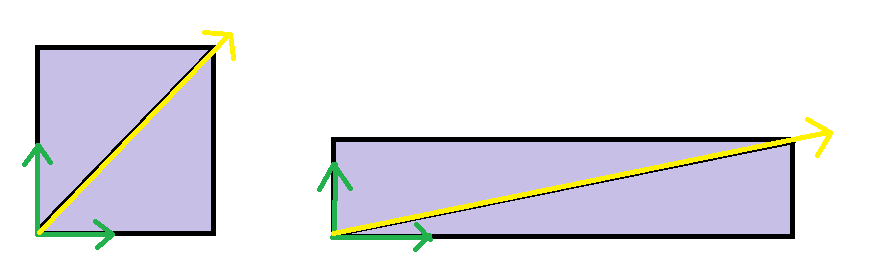
\includegraphics[width=7cm, height=1.5cm]{figures/pic.png}\\
\textcolor{Sepia}{EigenVectors are the green lines and arrows, and they don't change direction. Scaling is used here. Other vectors, such as the yellow one, do alter.
}}}


%----------------------------------------------------------------------------------------
%	RESULTS 1
%----------------------------------------------------------------------------------------

\headerbox{How to Find }{name=results,column=2,span=2,row=0}{

\begin{multicols}{2}
\vspace{1em}

\underline{\textcolor{Violet}{\textbf{How to Find Eigen values}}} \\
In order to determine a matrix's eigenvalues, take the following actions:

Verify that the specified matrix A is a square matrix  \\
1. Determine the same order's identity matrix I as well.\\
2. Calculate the matrix A-I in step two, where is a scalar value.\\
3. Locate the determinant of matrix A-I and set it equal to zero.\\
4. Determine all feasible values of, the necessary eigenvalues of matrix A, using the equation you've just created.



\vspace{4em}
\underline{\textcolor{Violet}{\textbf{How to Find Eigen vectors}}} \\
Follow the steps below to determine a matrix's eigenvectors:

Using the equation det ((A -\lambda   I) =0, 

where "I" is equivalent order identity 1.matrix as A, determine the eigenvalues of the provided matrix A. Indicate each of the eigenvalues  \lambda 1, \lambda 2, \lambda3.......    

2.In the formula AX =\lambda 1

or (A - \lambda1      I) X = 0, 

replace the numbers.\\
3.Determine the eigenvector X's value, which corresponds to the eigenvalue.\\
4.To obtain the eigenvector again for other eigenvalues, repeat the procedure.
\end{multicols}
}

%----------------------------------------------------------------------------------------
%	REFERENCES
%----------------------------------------------------------------------------------------

\headerbox{Submitted To}{name=references,column=0,above=bottom}{

\begin{description}\compresslist
\item[Name:] Md. Mohsinul Kabir
\item[Position:]  Assistant Professor
\item[Department:] Computer Science and Engineering
\end{description}
}


%----------------------------------------------------------------------------------------
%	CONTACT INFORMATION
%----------------------------------------------------------------------------------------

\headerbox{Submitted By}{name=contact,column=1,span=1,above=bottom}{ % This block is as tall as the references block

\begin{description}\compresslist
\item[Name:] Lomatul Mahzabin
\item[ID:]200042113
\item[Program:] Bsc in SWE
\item[Department:] Computer Science and Engineering
\end{description}
}

%----------------------------------------------------------------------------------------
%	CONCLUSION
%----------------------------------------------------------------------------------------

\headerbox{Study on Eigen Values and Eigen Vectors of Matrices }{name=conclusion,column=2,span=2,row=0,below=results}{

\begin{multicols}{2}
\begin{tikzpicture}[node distance=2.2cm]
\node (start1) [startstop] {\tiny KxK matrics has K egenvalues};
\node (dec1) [decision, below of=pro1] {\tiny are all the eigen value distinct?};
\node (pro2b1) [startstop1, right of=dec1, xshift=2cm] {\tiny There are K linearly independent eigenvectors};
\node (pro1) [process, below of=dec1] {\tiny For each Eigenvalue find algebric and geometric multiplicity};
\node (pro2) [process1, below of=pro1] {\tiny seaerch for defective eigenvalues};
\node (dec2) [decision, below of=pro2] {\tiny Is there any defective eigenvalue};
\node (pro2b2) [startstop1, right of=dec2, xshift=2cm] {\tiny There are K linearly independent eigenvectors};
\node (start2) [startstop,below of = dec2] {\tiny impossible to find K linearly independent eigenvectors};
\draw [arrow] (start1) -- (dec1);
\draw [arrow] (dec1)--node[anchor=south] {yes}(pro2b1);
\draw [arrow] (dec1)--node[anchor=east] {no}(pro1);
\draw [arrow] (pro1)--(pro2);
\draw [arrow] (pro2)--(dec2);
\draw [arrow] (dec2)--node[anchor=south] {no}(pro2b2);
\draw [arrow] (dec2)--node[anchor=east] {yes}(start2);
\end{tikzpicture}


Find the eigenvalues and eigenvectors for the matrix\\
A=
\begin{bmatrix}
5 & -10 & -5\\
2 & 14 & 2\\
-4 & -8 & 6
\end{bmatrix}

%------------------------------------------------
 First we need to find the eigenvalues of  A . Recall that they are the solutions of the equation\\
det (A -\lambda   I) =0

\begin{tabular}{ |p{3cm}|p{3cm}|}
\hline
Eigen Value & Eigen Vectors \\
\hline
 \lambda 1 = 5 & X1= \begin{bmatrix}
5 \\
-2\\
4
\end{bmatrix}  \\
\hline
\lambda 2 = 10 & X2= \begin{bmatrix}
-2 \\
1\\
0
\end{bmatrix}  \\
\hline
\lambda 3 = 10 & X3= \begin{bmatrix}
-1 \\
0\\
1
\end{bmatrix}  \\
\hline
\end{tabular}\\
\\
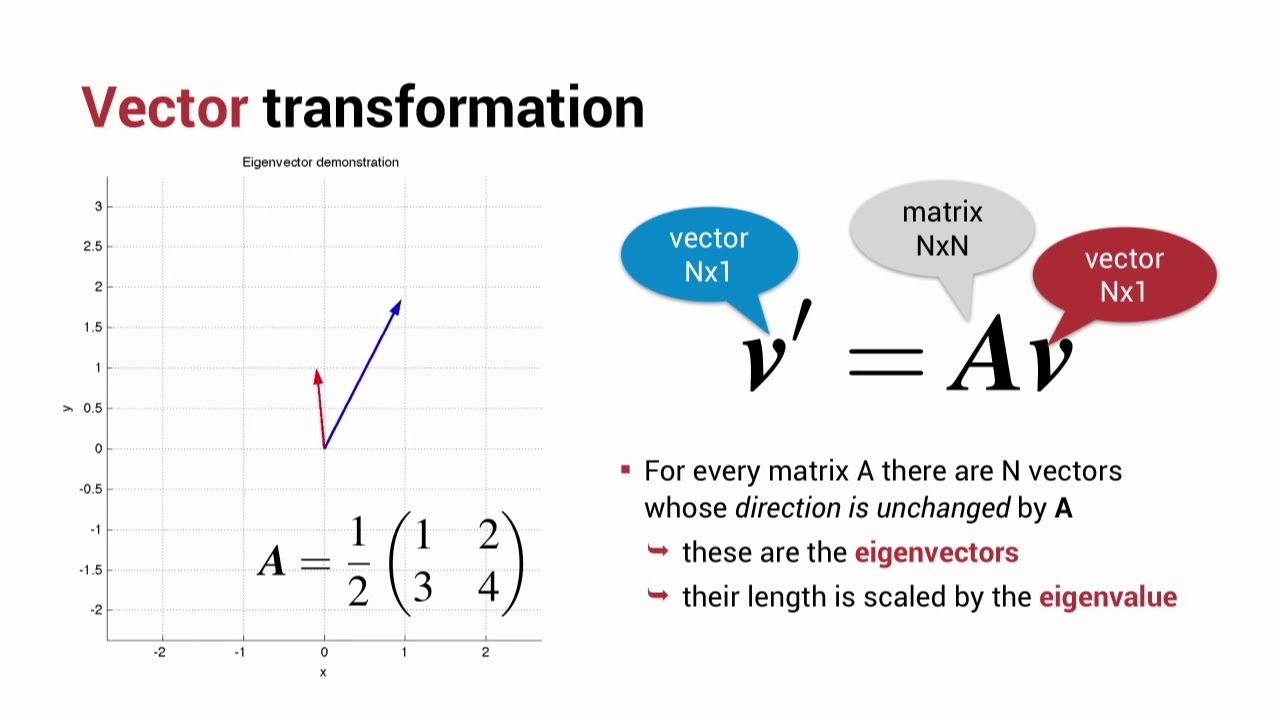
\includegraphics[width=7cm, height=3.5cm]{figures/pic 4.jpg}\\

\end{multicols}

}

%----------------------------------------------------------------------------------------
%	MATERIALS AND METHODS
%----------------------------------------------------------------------------------------

\headerbox{Applications}{name=method,column=0,below=abstract,span =2 ,below= introduction}{ % This block's bottom aligns with the bottom of the conclusion block
Eigenvalues and eigenvectors have a broad range of uses, including structural analysis, vibration, atomic orbitals, face recognition, and matrices diagonalization. They were first used to examine the principal axes of the rotary movement of rigid bodies.
\begin{itemize}\compresslist
\item \textcolor{Plum}{\textbf{Communication system:}}\\
The maximum amount of information that may theoretically be sent through a communication channel like the air or a phone line was calculated by Claude Shannon using eigenvalues. The communication channel's eigenvalues and eigenvectors (expressed as a matrix) are determined, and the eigenvalues are then waterfilled. The channel's fundamental modes are thus effectively represented by the eigenvalues, which are represented by the eigenvectors.
\item \textcolor{Plum}{\textbf{Bridge Building:}}\\
The natural frequency of the bridge is the smallest magnitude eigenvalue of a system that simulates the bridge. This information is used by engineers to ensure the stability of their structures.
\item\textcolor{Plum}{\textbf{ Design of Automotive Stereo Systems:}}\\
Additionally, eigenvalue analysis is applied in the development of automotive radio systems to improve the reproduction of musically-induced vehicle vibration.
\item\textcolor{Plum}{\textbf{ Electrical Engineering:}}\\
It is desirable to decouple three-phase systems using symmetrical component transformation using eigenvalues and eigenvectors.
\end{itemize}
}





\headerbox{Diagonalization and the eigendecomposition}{name= projection,column=0,below=abstract,span =2 ,below=method}{ % This block's bottom aligns with the bottom of the conclusion block
Sometimes referred to as Eigenvalue Decomposition, Eigen Decomposition (shortcut EVD)
\begin{itemize}\compresslist
\item {is a technique for diagonalizing a square n-by-n matrix A.}
\item {Using eigenvectors, we may transform a matrix into a diagonal matrix.}
\end{itemize}\\
An "canonical form" is created by decomposing a matrix into its eigenvalues.
\begin{itemize}\compresslist
\item{From a given diagonal matrix, we wish to create a smaller one.}
\item{If a matrix A resembles a diagonal matrix, it can be diagonalized.a matrix A is similar to B if there exists an invertible M s.t. B=M^{-1}AM}

\item{A is diagonalizable if there exists invertible matrix P s.t. P^{-1}AP 

is diagonal.}


\end{itemize}
}
\headerbox{Conclusion}{name= projection,column=2,below=abstract,span =2 ,below=conclusion,above=bottom}{ % This block's bottom aligns with the bottom of the conclusion block
As expected, eigenvalues are the values of the extension factor associated with an eigenvector, which is a vector whose direction does not change after being transformed by a given T.

In additional detail, eigenvectors are vectors that are not trivial and are hence distinct from 0.
Eigenvalues are a unique collection of scalar values connected to a set of linear equations that are most likely seen in matrix equations. The characteristic roots are another name for the eigenvectors. It is a non-zero vector that, after applying linear transformations, can only be altered by its scalar component.Eigenvalues display the system's strength in the direction of the relevant eigenvector. The physical property that the provided matrix represents determines the relevance of the eigenvalues and eigenvectors in terms of physics.

}
\end{poster}

\end{document}